\documentclass[border=2pt]{standalone}

% Drawing
\usepackage{tikz}

% Notation
\usepackage{physics}

% Tikz Library
\usetikzlibrary{calc}

% Newcommand
%% Point
\newcommand{\point}[1]{\draw[fill=black] (#1) circle (1.5pt);}
%node [shift={(#3)}] {#2};

% Style
\tikzset{mass/.style={inner sep = 2.2pt, circle}}

\begin{document}
	
	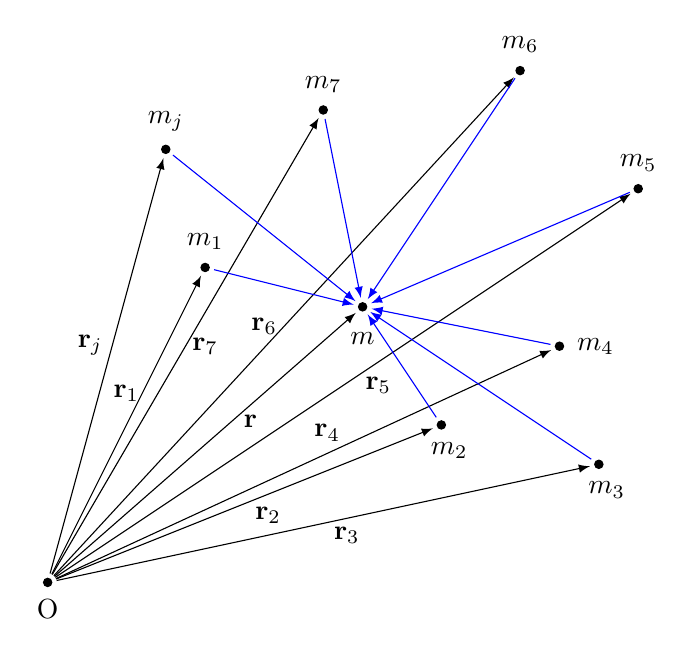
\begin{tikzpicture}
		%Grid
%		\draw[thin, dotted] (0,0) grid (8,8);
%		\foreach \i in {1,...,8}
%		{
%			\node at (\i,-2ex) {\i};	
%		}
%		\foreach \i in {1,...,8}
%		{
%			\node at (-2ex,\i) {\i};	
%		}
%		\node at (-2ex,-2ex) {0};
		
		% Coordiantes
		\node[mass] (O) at (0,0) {};
		\node[mass] (A) at (4,3.5) {};
		\node[mass] (B1) at (2,4) {};
		\node[mass] (B2) at (5,2) {};
		\node[mass] (B3) at (7,1.5) {};
		\node[mass] (B4) at (6.5,3) {};
		\node[mass] (B5) at (7.5,5) {};
		\node[mass] (B6) at (6,6.5) {};
		\node[mass] (B7) at (3.5,6) {};
		\node[mass] (Bj) at (1.5,5.5) {};
		\node (a) at ($(O)!0.5!(A)$) {};
		\foreach \i in {1,...,7}
		{
			\node (b\i) at ($(O)!0.5!(B\i)$) {};
		}
		
		% Points
		\point{O}
		\point{A}
		\foreach \i in {1,...,7}
		{
			\point{B\i}
		}
		\point{Bj}
		
		% Vectors
		\draw[-latex] (O) -- (A) node [pos=0.65, below] {$\vb{r}$};
		\foreach \i in {1,...,7}
		{
			\draw[-latex] (O) -- (B\i);
		}
		\draw[-latex] (O) -- (Bj) node [pos=0.55, left] {$\vb{r}_j$};
		%
		\foreach \i in {1,...,7}
		{
			\draw[-latex, blue] (B\i) -- (A);
		}
		\draw[-latex, blue] (Bj) -- (A);
		
		% Nodes
		\node[below, shift={(0,-0.1)}] at (O) {$\mathrm{O}$};
		%% Masses
		\node[below, shift={(0,-0.2)}] at (A) {$m$};
		\node[above, shift={(0,0.1)}] at (B1) {$m_1$};
		\node[below, shift={(0.1,-0.1)}] at (B2) {$m_2$};
		\node[below, shift={(0.1,-0.1)}] at (B3) {$m_3$};
		\node[right, shift={(0.1,0)}] at (B4) {$m_4$};
		\node[above, shift={(0,0.1)}] at (B5) {$m_5$};
		\node[above, shift={(0,0.1)}] at (B6) {$m_6$};
		\node[above, shift={(0,0.1)}] at (B7) {$m_7$};
		\node[above, shift={(0,0.1)}] at (Bj) {$m_j$};
		%% Vectors
		\node[shift={(0,0.4)}] at (b1) {$\vb{r}_1$};
		\node[shift={(0.3,-0.15)}] at (b2) {$\vb{r}_2$};
		\node[shift={(0.3,-0.15)}] at (b3) {$\vb{r}_3$};
		\node[shift={(0.3,+0.4)}] at (b4) {$\vb{r}_4$};
		\node[shift={(0.45,0)}] at (b5) {$\vb{r}_5$};
		\node[shift={(-0.25,0)}] at (b6) {$\vb{r}_6$};
		\node[shift={(0.25,0)}] at (b7) {$\vb{r}_7$};
	\end{tikzpicture}
	
\end{document}